    In this chapter, we introduce the three main information measures (entropy, relative entropy, and mutual information) for discrete distributions with finite support. We begin this chapter with a simple guessing game, which naturally leads the definition of these three terms, and we then study some simple properties of these information measures. 

    \emph{Notation.} As mentioned earlier, throughout this chapter, we will work with discrete distributions supported on a finite set, which we denote by $\X$. The elements of this set could be anything, and in particular, we do not assume that there exists any ordering among them. We will mostly consider $\log$ to the base $2$, unless otherwise stated. 

    \section{A Guessing Game}
    \label{sec:guessing-game}
        We consider a collection of simple guessing games (or a 20 questions games)  that will motivate the definitions of the three main information measures: entropy, relative entropy, and mutual information. 

       \begin{question}[Guessing Game I] 
           \label{question:binary-search-game}
           In the simplest setting, suppose there are $n$ identical bins, and a ball is placed uniformly at random in one of the bins. Denote the position of the ball with the random variable $X \sim \text{Uniform}\lp \mc{X} \rp$, where $\mc{X} = \{0, 1, \ldots, n-1\}$. Suppose, we can make binary queries of the form: \emph{``Is $X$ in the set $A$?''} for $A \subset \mc{X}$.  Our objective is to design a strategy of asking a series of such questions, such that the average number of questions required to identify the bin containing the ball~(i.e., the value of the random variable $X$) is small. 
       \end{question} 

        A simple strategy could be to ask the series of questions: is $X=0$, is $X=1$, and so on. With this strategy, we can check that the average number of questions needed are equal to 
        \begin{align}
            L = \sum_{i=0}^{n-1} \mathbb{P}(X=i) (i+1) = \frac{1}{n} \sum_{i=0}^{n-1} (i+1) = \frac{1}{n} \lp 1 + 2 + \ldots + n\rp = \frac{n}{2}. 
        \end{align}
        Thus, the number of yes/no questions required by this strategy~(called the linear search) is $\Omega(n)$. This strategy is quite inefficient, since with every query we reduce the search space by one. As we see next, we can do significantly better. 

         An optimal strategy for the above problem is the \emph{binary search}, in which the queries are specifically designed to reduce the size of search space by half with each query.  In particular, consider the case of $n=4$. Then, the binary search decision tree is shown in~\Cref{fig:binary-search}. Assigning the values $0 \leftarrow Y$ and $1\leftarrow N$, we see that the series of questions to ascertain a value of $X=i$ is equivalent to the binary encoding or representation of $i$. 
         \begin{align}
             0  \equiv (YY) \equiv (00), \quad 
             1  \equiv (YN) \equiv (01), \quad 
             2  \equiv (NY) \equiv (10), \quad
             3  \equiv (NN) \equiv (11) . 
         \end{align}
         

        \begin{figure}[hbt!]
            \centering
            \def\figwidth{0.5\columnwidth}
            \def\figheight{0.25\columnwidth} % Feel free to change
            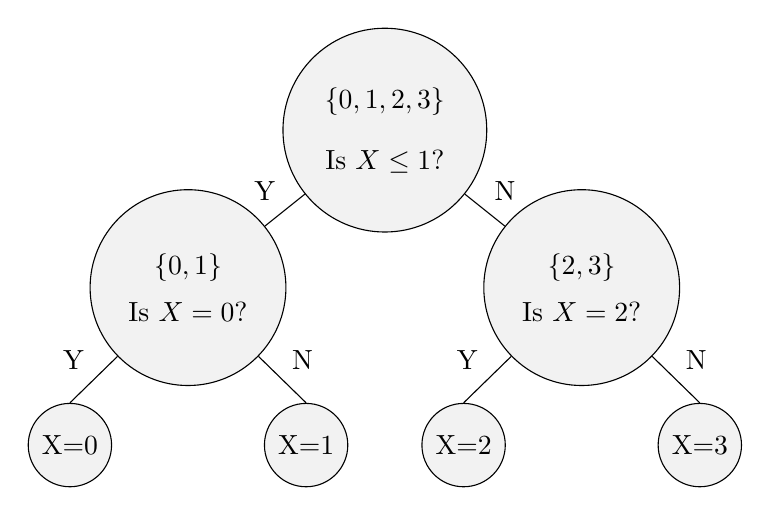
\begin{tikzpicture}[
  decision node/.style={draw, circle, minimum size=1cm, fill=gray!10},
  leaf node/.style={draw, circle, minimum size=1cm, fill=gray!10},
  level distance=1.5cm,
  level 1/.style={sibling distance=4cm},
  level 2/.style={sibling distance=2cm}
]
  % Root node
  % \node[decision node] (root) at (0, 0) {$\{1, 2, 3, 4\}$};
  \node[decision node] (root) at (0, 0) {%
    \parbox{2cm}{\centering $\{0, 1, 2, 3\}$ \\ \vspace{1em} \red{Is $X \leq 1$?}}
  };

  
  % Left child of the root
  \node[decision node] (left) at (-2.5, -2) {%
    \parbox{2cm}{\centering $\{0, 1\}$ \\ \vspace{0.5em} \red{Is $X=0$?}}
  };
  % Right child of the root
  \node[decision node] (right) at (2.5, -2) {%
    \parbox{2cm}{\centering $\{2, 3\}$ \\ \vspace{0.5em} \red{Is $X=2$?}}
  }; 
  % Leaves
  \node[leaf node] (x1) at (-4, -4) {X=0};
  \node[leaf node] (x2) at (-1, -4) {X=1};
  \node[leaf node] (x3) at (1, -4) {X=2};
  \node[leaf node] (x4) at (4, -4) {X=3};
  
  % Edges
  \draw (root) -- node[above left] {Y} (left);
  \draw (root) -- node[above right] {N} (right);
  
  % Edges from the left child
  \draw (left) -- node[above left] {Y} (x1.north);
  \draw (left) -- node[above right] {N} (x2.north);
  
  % Edges from the right child
  \draw (right) -- node[above left] {Y} (x3.north);
  \draw (right) -- node[above right] {N} (x4.north);
\end{tikzpicture}

            \caption{The figure shows the decision tree for the optimal strategy~(i.e., binary search) for the guessing game with $X$ drawn uniformly at random from $\mc{X} = \{0, 1, 2, 3\}$. Each query is chosen to ensures that the outcomes (i.e., Y or N) are equiprobable. In other words, this strategy proceeds by greedily selecting a query whose outcome is the most uncertain.}
            \label{fig:binary-search}
        \end{figure}
  
        Denote the number of questions needed to verify $X=i$ by $\ell_i$. Then, the binary search scheme asks $\ell_i=2$ questions for all $i \in \mc{X}$~(in other words, it represents each $i \in \mc{X}$ with a \emph{codeword} of length $\ell_i=2$). Interestingly, $2$ is also equal to  the negative of the logarithm of the probability assigned to each value $i \in \mc{X}$ to the base $2$; that is, $2 = \log(1/p_i) = \log(4)$. The average number of questions required by this (optimal) strategy is then equal to
        \begin{align}
            L = 2 = \sum_{i=0}^{3} p_i \ell_i = \sum_{i=0}^3 p_i \log (1/p_i). 
        \end{align}
        Thus, the above discussion suggests that the number of binary questions needed to completely remove the uncertainty about the value of $X \sim Uniform(\mc{X})$ is $\log(|\mc{X}|)$. What is the analog of this quantity for  non-uniform distribution over $\mc{X}$? We consider this question in the next version of the guessing game. 
% 
        \begin{question}[Guessing game II] 
            \label{question:guessing-game-II}
            Consider the same setting as~\Cref{question:binary-search-game} with $\mc{X} = \{0, 1, 2, 3\}$, but assume that $X$ is drawn from the following distribution (instead of uniformly): 
            \begin{align}
                P_X = (p_0, p_1, p_2, p_3) = \lp \frac{1}{8}, \frac{1}{8}, \frac{1}{4}, \frac{1}{2} \rp. 
            \end{align}
            What is the optimal sequence of binary questions to identify the true value of $X$? 
        \end{question}

        We will develop a strategy for this problem, motivated by the 'halving' property of the binary search scheme for the uniform case. In particular, we will take the strategy which can be summarized as follows: 
        \begin{quote}
            \centering
                \emph{make queries whose outcomes are equally likely (or in other words, are most uncertain).}
        \end{quote}
        Note that when $X$ is uniformly distributed, the above strategy reduces exactly to the binary search. 
        The decision tree of this strategy for the distribution of~\Cref{question:guessing-game-II} is shown in~\Cref{fig:guessing-game-II}. Unlike the previous game, the decision tree is not balanced --- it asks more questions of the less likely values of $i$. The expected number of questions in this case is equal to 
        \begin{align}
            L &= \sum_{i=0}^3 p_i \ell_i = \frac{1}{8}\times 3 + \frac{1}{4} \times 2  + \frac{1}{4} \times 2 + \frac{1}{2} \times 1 = \frac{15}{8} \\
            & = -\sum_{i=1}^n p_i \log p_i \defined H(P_X). 
        \end{align}
        Again the average number of yes/no questions needed to learn $X$ is characterized by the quantity, $-\sum_{i \in \mc{X}} p_i \log p_i$. This functional of the probability distribution is called its \emph{entropy}, also called its self-information. As we will see later, it is a fundamental limit  on the average number of yes/no questions needed to learn the value of $X$~(or equivalently, the average length of a binary lossless representation of all realizations of $X$).   

        \begin{figure}[hbt!]
            \centering
            \def\figwidth{0.5\columnwidth}
            \def\figheight{0.25\columnwidth} % Feel free to change
            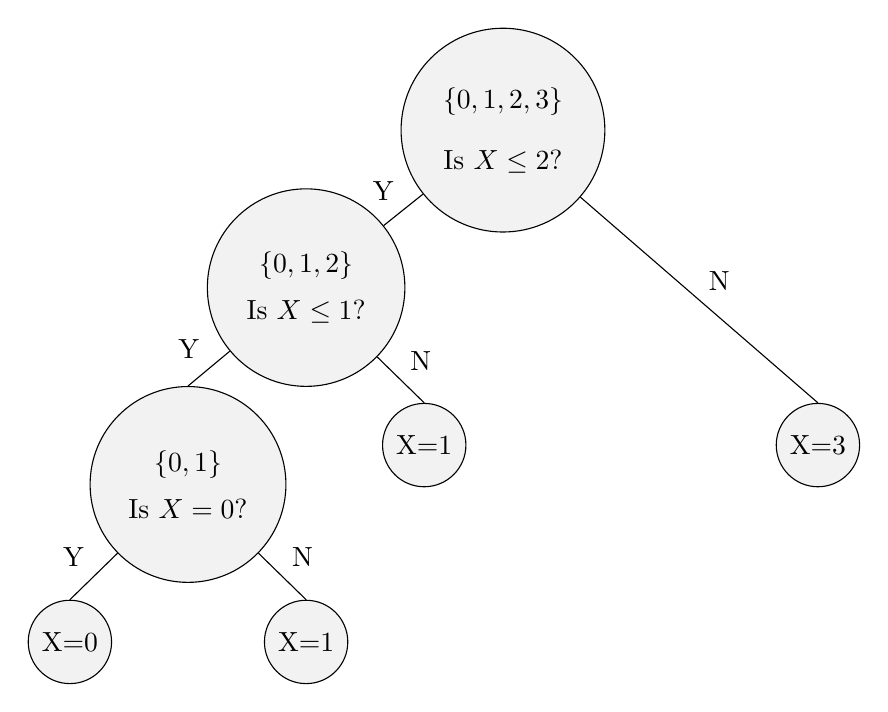
\begin{tikzpicture}[
  decision node/.style={draw, circle, minimum size=0.25cm, fill=gray!10},
  leaf node/.style={draw, circle, minimum size=1cm, fill=gray!10},
  level distance=1.5cm,
  level 1/.style={sibling distance=4cm},
  level 2/.style={sibling distance=2cm}
]
  % Root node
  % \node[decision node] (root) at (0, 0) {$\{1, 2, 3, 4\}$};
  \node[decision node] (root) at (0, 0) {%
    \parbox{2cm}{\centering $\{0, 1, 2, 3\}$ \\ \vspace{1em} \red{Is $X \leq 2$?}}
  };

  
  % Left child of the root
  \node[decision node] (left) at (-2.5, -2) {%
    \parbox{2cm}{\centering $\{0, 1, 2\}$ \\ \vspace{0.5em} \red{Is $X\leq 1$?}}
  };
  
  \node[decision node] (x1) at (-4, -4.5) {%
    \parbox{2cm}{\centering $\{0, 1\}$ \\ \vspace{0.5em} \red{Is $X=0$?}}
  };

  
  \node[leaf node] (x2) at (-1, -4) {X=1};
  % \node[leaf node] (x3) at (1, -4) {X=2};
  \node[leaf node] (x4) at (4, -4) {X=3};
  \node[leaf node] (x5) at (-5.5, -6.5) {X=0};
  \node[leaf node] (x6) at (-2.5, -6.5) {X=1};

  
  % Edges
  \draw (root) -- node[above left] {Y} (left);
  % \draw (root) -- node[above right] {N} (right);
  
  % Edges from the left child
  \draw (left) -- node[above left] {Y} (x1.north);
  \draw (left) -- node[above right] {N} (x2.north);

    % Edges from the left child
  \draw (x1) -- node[above left] {Y} (x5.north);
  \draw (x1) -- node[above right] {N} (x6.north);
 
  
  % Edges from the right child
  % \draw (root) -- node[above left] {Y} (x3.north);
  \draw (root) -- node[above right] {N} (x4.north);
\end{tikzpicture}

            \label{fig:guessing-game-II}
            \caption{The figure shows the decision tree for the optimal strategy for a non-uniform probability distribution over $\X$. The key observation is that this strategy assigns fewer questions (or a shorter codeword) to the higher probability symbol~($3$), and more questions to the less probable symbols, such as $0$ and $1$.}
        \end{figure}

        In both the previous games, we assumed that the player knows the true distribution of $X$ exactly. We now consider a situation where there is a mismatch between the true and the assumed distribution of $X$. 
        \begin{question}
            \label{question:guessing-game-III}
            Consider the same setting as~\Cref{question:guessing-game-II}, but now assume that the true distribution $(P_X)$ of $X$ is not known to the player, and instead he believes that $X \sim Q_X$, where $Q_X = (1/2, 1/8, 1/8, 1/4)$. What is the effect of this distribution mismatch? 
        \end{question}

        Under the assumption that the true distribution is $Q_X$, the optimal codeword assignment is 
        \begin{align}
            0 \equiv (Y) \equiv (0), \quad 
            1 \equiv (NNY) \equiv (110), \quad 
            2 \equiv (NNN) \equiv (111), \quad 
            3 \equiv (NY) \equiv (10). 
        \end{align}
        Again, as before, in this example, the number of questions needed to ascertain that $X=i$ is equal to $\log(1/q_i)$. The average number of questions needed to learn the value of $X$ is 
        \begin{align}
            L &= \sum_{i=0}^3 p_i \log(1/q_i) = - \sum_{i=1}^3 p_i\log(p_i) +  \sum_{i=0}^3 p_i \log(p_i/q_i)  \\
            & = H(P_X) + \dkl(P_X \parallel Q_X). 
        \end{align}
        The second term in the display is called the relative entropy or KL divergence between $P_X$ and $Q_X$, and it denotes the price paid by the player for using the wrong model for asking the yes/no questions~(or the extra average codeword length incurred due to the ignorance of the true distribution). As we will see later, this quantity is always non-negative. 

        \begin{question}
            \label{question:guessing-game-IV} Finally, we now consider a case of guessing another random variable $Y$ on the set $\{a, b\}$. The joint distribution of $X$ and $Y$ is stated in~\Cref{tab:joint-distribution}.  

            Suppose we want to ask a series of yes/no questions to find out the true value of both $X$ and $Y$. Consider two strategies: 
            \begin{itemize}
                \item Player 1 develops two  independent strategies for learning $X$ and $Y$ 
                \item Player 2 develops a joint strategy for learning $X$ and $Y$ together. 
            \end{itemize}
            Who does better in terms of the average number of questions needed to learning both $X$ and $Y$? How much is the improvement? 
        \end{question}
        \begin{table}
            \centering
            \begin{tabular}{|c|c|c|c|c|}
                \hline
                & $X=0$ & $X=1$ & $X=2$ & $X=3$  \\
            $Y=a$& 0 & 1/8 & 1/8 & 0 \\
            $Y=b$& 1/8 & 0 & 1/8 & 1/2  \\ 
            \hline 
            \end{tabular}
            \caption{Joint distribution $P_{XY}$ of $(X, Y)$.}
            \label{tab:joint-distribution}
        \end{table}

        From the table, we can check that $Y$ has a distribution $P_Y = (1/4, 3/4)$ over the set $\{a, b\}$. The marginal distribution of $X$ is the same as in the previous two questions. Hence, we expect that the average number of yes/no questions need by player 1~(denoted by $L_1$) is 
        \begin{align}
            L_1 = H(P_X) + H(P_Y) \approx 1.75 + 0.811 \text{ bits} = 2.561 \text{ bits}
        \end{align}
        For the second player, who develops a joint strategy for querying about $(X, Y)$, we expect the average number of yes/no questions~(denoted by $L_2$) to be 
        \begin{align}
            L_2 = H(P_X, P_Y) = 4\times \frac{1}{8}\times 3 + \frac{1}{2} \times 1 = 2 \text{ bits}. 
        \end{align}
        Thus, the player who jointly considers the two random variables requires fewer questions. This is because, knowing the value of $Y$ also provides information about the $X$ value. For instance, if we know that $Y=a$, then we know that $X$ cannot be $0$ or $3$. Exploiting this leads to the reduced number of questions needed by player 2. The amount of improvement, $L_1 - L_2$, is equal to 
        \begin{align}
            L_1 - L_2 = H(X) + H(Y) - H(X, Y) \defined I(X; Y). 
        \end{align}
        The term $I(X; Y)$ is called the \emph{mutual information} between the random variables $X$ and $Y$, and it precisely quantifies the amount of information that $X$ contains about $Y$~(or equivalently, $Y$ contains about $X$; since $I(X; Y)$ is symmetric).  

        \paragraph{Summary.} The above discussion can be summarized as follows:
        \begin{itemize}
            \item Entropy $H(X) = -\sum_{i} p_i \log(p_i)$ quantifies the information content of a random variable $X$. It is also equal to the minimum average number of yes/no questions needed to learn the value of $X$. 
            \item The relative entropy is a measure of discrepancy between two distributions $P_X$ and $Q_X$. It quantifies the additional (on an average) number of yes/no questions needed to learn about $X$, under wrong model assumptions. 
            \item The mutual information $I(X; Y)$ is measure of dependence between $X$ and $Y$. It quantifies how much information about $X$ is contained in the random variable $Y$. 
        \end{itemize}
        
    \section{Formal Definitions}
        In this section, we formally define the three information measures, and observe some of their basic properties. The next section contains a more thorough treatment of the properties of these measures. 
        
        \begin{definition}
            \label{def:entropy-discrete}
            Suppose $X$ denotes an $\X$-valued random variable with  probability mass function~(\pmf) $p_X$. Then, the entropy of $X$~(actually the distribution $p_X$) is defined as 
            \begin{align}
                H(X) \equiv H(p_X) = \sum_{x \in \X} -p_X(x) \log(p_X(x)). \label{eq:disc-entropy-def-1}
            \end{align}
            For a pair of distributions $(X, Y)$ on $\X \times \X$ with joint distribution $p_{XY}$, their joint entropy is defined as, following~\eqref{eq:disc-entropy-def-1}, 
            \begin{align}
                H(X, Y) \equiv H(p_{XY}) = \sum_{x \in \X} \sup_{y \in \X} -p_{XY}(x, y) \log( p_{XY}(x, y)). 
            \end{align}
            Finally, the conditional entropy of $X$ given $Y$ is defined as the average (over the marginal $p_X$) of the entropy of $Y|X=x$. That is, 
            \begin{align}
                H(Y|X) \equiv H(p_{Y|X}|p_X) = \sum_{x \in \mc{X}} p_X(x) \sum_{y \in \X} -p_{Y|X}(y|x) \log \lp p_{Y|X}(y|x) \rp. 
            \end{align}
        \end{definition}


        \begin{remark}
            \label{remark:unit-entropy}
            The base of the logarithm used in defining the entropy characterizes its unit: if the base is $2$, entropy is measured in \emph{bits}, while for natural logarithm with base $e$, the unit is called \emph{nats}. It is easy to verify that changing the base from $a$ to $b$ is achieved by the simple identity: $H_a(X) = \log_b a H_b(X)$. 
        \end{remark}    
        % 
        Entropy is defined as a quantitative measure of the amount of `uncertainty' contained in a probability distribution. In fact, there exist several results that begin by stating a set of reasonable axioms to be satisfied by a good measure of uncertainty, and then prove that the above definition is the only one that simultaneously satisfies those properties~\citep{csiszar2011information}. 

        We can also intuitively see that the above definition serves as a good measure of uncertainty. For instance, suppose $\X = \{0, 1\}$ and $X$ is a Bernoulli distribution with parameter $p$. Then, the entropy of $X$, also called binary entropy, and denoted by $h_2(p)$, is defined as 
        \begin{align}
            h_2(p) = -p \log (p) - \bar{p} \log \bar{p}, \quad \text{where } \bar{p} \coloneqq 1 - p. 
        \end{align}
        On plotting it, we can see that the $h_2(p)$ is zero at $p \in \{0, 1\}$, and it achieves its maximum at $p=1/2$. 

        \begin{figure}
            \centering
              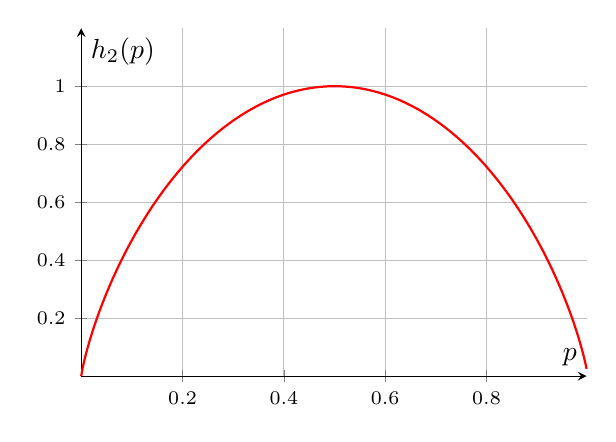
\begin{tikzpicture}
    \begin{axis}[
        xlabel=$p$,
        ylabel=$h_2(p)$,
        domain=0:1,
        samples=400,
        ymin=0,
        ymax=1.2,
        width=8cm,
        height=6cm,
        axis lines=middle,
        grid=major,
        clip=false,
        xtick={0, 0.2, 0.4, 0.6, 0.8, 1},
        ytick={0, 0.2, 0.4, 0.6, 0.8, 1},
        tick label style={font=\scriptsize},
        legend style={at={(0.95,0.95)},anchor=north east, font=\scriptsize},
    ]
    \addplot [red, thick] {-x * log2(x) - (1 - x) * log2(1 - x)};
    \end{axis}
\end{tikzpicture} 
            \caption{Variation of the binary entropy $h_2(p) = -p \log(p) - \bar{p} \log(\bar{p})$ with the parameter $p$. Note that $h_2(p)$ is zero for $p \in \{0, 1\}$, when the random variable is deterministic, and is maximized at $p=0.5$, which corresponds to the maximum uncertainty. Also note that the qualitative behavior of the curve is similar to that of the variance $p(1-p)$; another measure of dispersion or variability of the distribution.}
            \label{fig:binary-entropy}
        \end{figure}

        The definition of entropy leads to some immediate conclusions that we record next: 
        \begin{proposition}
            The following statements are true for $\X$-valued random variables $X, Y$ etc.: 
            \begin{enumerate}[label=(\alph*)]
                \item  $H(X) \geq 0$, for all random variables $X$, and its minimum value of $0$ is achieved if and only if $X$ is equal to a constant with probability $1$. 
                \item The joint entropy of $(X, Y)$ is equal to the entropy of $X$, plus the conditional entropy of $Y$ given $X$:
                \begin{align}
                    H(X, Y) = H(X) + H(Y|X) = H(Y) + H(X|Y). 
                \end{align}
                \item For any function $f: \X \to \X$, we have $H(f(X)) \leq H(X)$, with equality iff $f$ is bijective. 
            \end{enumerate}
        \end{proposition}

        \begin{proof}
            \begin{enumerate}[label=(\alph*)]
                \item Since $H(X) = \sum_{x \in \X} p(x) \log 1/p(x)$, it is a sum of non-negative terms, which implies that $H(X) \geq 0$. To achieve the equality, note that each $p(x) \log 1/p(x)$ must be equal to zero; which implies that for all $x \in \X$, the value of $p(x)$ must lie in $\{0, 1\}$. Since $\sum_{x \in \X} p(x)$ is constrained to be equal to $1$, the result follows. 
                
                \item This follows directly by the definition of joint and conditional entropies. In particular, 
                \begin{align}
                    H(X, Y) &= \sum_{x, y} -p(x, y) \log p(x,y) = -\sum_{x \in \X} p(x) \sum_{y \in \Y} p(y|x) \big( \log p(x) + \log p(y|x) \big)  \\
                    & = - \sum_{x \in \X} p(x) \log p(x) \sum_{y \in \Y} p(y|x) - \sum_{x \in \X} p(x) \sum_{y \in \Y} p(y|x) \log p(y|x) \\
                    & = H(X) + H(Y|X). 
                \end{align}
                Repeating the same argument, but now writing $p(x, y) = p(y) p(x|y)$, we get the other equivalent definition. 
                \item This is a simple consequence of the previous two results. In particular, we set $Y = f(X)$. Then, 
                \begin{align}
                    H(Y) + H(X|Y) = H(X, Y) = H(X) + H(Y|X) = H(X), 
                \end{align}
                where the last equality is a consequence of the fact that $Y = f(X)$; and hence $H(Y|X)$ is equal to $0$. Since $H(X|Y)$ is not necessarily zero, we get the required inequality $H(Y) \leq H(X)$. In words, this means that we cannot add more uncertainty (or self-information) to a signal by applying a deterministic function. 
            \end{enumerate}
        \end{proof}

        We now present a simple application of the law of large numbers to characterize the support of a high dimensional product distribution in terms of the entropy.
        \begin{proposition}[Asymptotic equipartition probability~(AEP]
            \label{prop:discrete-AEP} 
            Let $X_1, X_2, \ldots, X_n \simiid P_X$, and for a fixed $\epsilon >0$, define the `typical set' $A_n(\epsilon)$ as 
                \begin{align}
                    A_n(\epsilon) = \lbr x^n\in \X^n: 2^{-n\lp H(X) - \epsilon \rp} \leq \mathbb{P}(X^n) = \prod_{i=1}^n P_X(X_i) \leq 2^{-n\lp H(X) + \epsilon \rp} \rbr. \label{eq:typical-set-1}
                \end{align}
                Then, the following statements are true: 
                \begin{itemize}
                    \item $\lim_{n \to \infty} \mathbb{P}(A_n(\epsilon)) = 0$. 
                    \item $|A_n(\epsilon)| \leq 2^{n(H(X) + \epsilon)}$. 
                    \item For $n$ large enough, we have $|A_n(\epsilon)| \geq (1-\epsilon)2^{n(H(X)-\epsilon)}$. 
                \end{itemize}
            Thus, for large $n$, a small subset $A_n(\epsilon)$ of $\X^n$, consisting of roughly equiprobable sequences, contains almost all the probability. 
        \end{proposition}
        \begin{proof}
            \begin{itemize}
                \item This is simply an application of the weak LLN to $-\log(\mathbb{P}(X^n))$.  
                \item We prove this by noting that $\mathbb{P}(A_n(\epsilon))\leq 1$, and thus 
                \begin{align}
                    1 & \geq \sum_{x^n \in A_n(\epsilon)} \mathbb{P}(x^n) \geq \sum_{x^n \in A_n(\epsilon)} 2^{-n H(X) - n\epsilon} = |A_n(\epsilon)|2^{-n H(X) - n\epsilon}. 
                \end{align}
                \item By the definition of convergence in probability, for $n$ large enough, we have $\mathbb{P}(A_n(\epsilon)) \geq 1-\epsilon$. Hence, we have 
                \begin{align}
                    1-\epsilon & \leq \mathbb{P}\lp A_n(\epsilon) \rp = \sum_{x^n \in A_n(\epsilon)} \mathbb{P}(x^n) \leq \sum_{x^n \in A_n(\epsilon)} 2^{-n(H(X) - \epsilon)} = |A_n(\epsilon)| 2^{-n(H(X) - \epsilon)}. 
                \end{align}
            \end{itemize}
        \end{proof}
        \begin{remark}
            \label{remark:aep-1} The above result can be used to construct a theoretically simple, but computationally infeasible, compression scheme. The idea is simple: enumerate all elements of $x^n \in A_n(\epsilon)$,  and assign them their binary representation prefixed by an additional `$0$' as the codeword; and for all points in $A_n(\epsilon)^c$, assign a codeword starting with `$1$', followed by the binary representation after enumerating all elements. It is easy to check that this lossless compression scheme has an average codeword length (per symbol) smaller than $H(X) + (2+\epsilon + \log(|\X|))/n$.  
        \end{remark}

        The next, and perhaps the most important, information measure that we introduce is the relative entropy, also known as the Kullback-Leibler or KL divergence. 
        \begin{definition}[Relative Entropy]
            \label{def:relativ-entropy}
            The relative entropy between two distributions $P_X$ and $Q_Y$ on the same domain $\X$ is defined as 
            \begin{align}
                \dkl(P_X \parallel Q_Y) = \sum_{x \in \X} p(x) \log \lp \frac{ p(x)}{q(x)} \rp.  
            \end{align}
            For joint distributions $P_{XY}$ and $Q_{XY}$, the conditional relative entropy is defined as 
            \begin{align}
                \dkl\lp  P_{Y|X} \parallel Q_{Y|X} \vert P_X \rp = \sum_{x \in \mc{X}}p(x) \sum_{y \in \mc{Y}} p(y|x) \log \lp \frac{p(y|x)}{q(y|x)} \rp = \sum_{x \in \mc{X}} p(x) \dkl\lp P_{Y|X=x} \parallel Q_{Y|X=x} \rp. 
            \end{align}
            In other words, the conditional relative entropy is the average (over the marginal $P_X$) relative entropy between the conditional distributions $P_{Y|X=x}$ and $Q_{Y|X=x}$. 
        \end{definition}
        From the definition we can see that the relative entropy is not symmetric in its arguments. As an example, consider the two ways of computing the  relative entropy between $X \sim \text{Bernoulli}(p)$ and $Y \sim \text{Bernoulli}(1/2)$, as plotted in~\Cref{fig:binary-kl}. 
        \begin{figure}
            \centering
            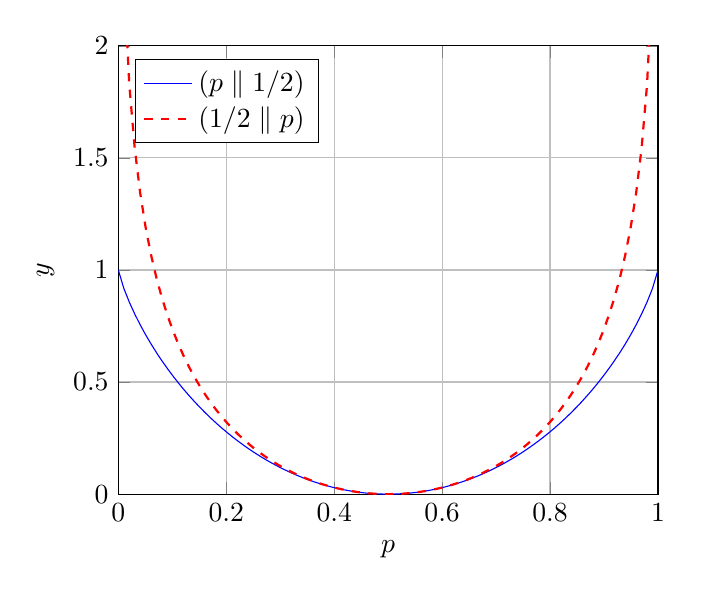
\begin{tikzpicture}
  \begin{axis}[
    xlabel=$p$,
    ylabel=$y$,
    xmin=0, xmax=1,
    ymin=0, ymax=2,
    legend pos=north west,
    grid=both,
    ]
    
    % Function  p * log2(2 * p) + (1 - p) * log2(2 * (1 - p))
    \addplot[blue, domain=0:1, samples=100] {x * log2(2 * x) + (1 - x) * log2(2 * (1 - x))};
    \addlegendentry{$\dkl(p \parallel 1/2)$}
    
    % Function 0.5 * (log2(1 / (2 * p)) + log2(1 / (2 * (1 - p))))
    \addplot[red, domain=0:1, samples=100, dashed, thick] {0.5 * (log2(1 / (2 * x)) + log2(1 / (2 * (1 - x))))};
    \addlegendentry{$\dkl(1/2 \parallel p)$}
    
  \end{axis}
\end{tikzpicture}

            \caption{Plots of  $\dkl(P_X\parallel P_Y)$ and $\dkl(P_Y\parallel P_X)$, where $X \sim \text{Bernoulli}(p)$ and $X \sim \text{Bernoulli}(1/2)$, as $p$ varies in $[0,1]$. The figures illustrates the locally quadratic behavior of relative entropy, and also shows that it is not symmetric.}
            \label{fig:binary-kl}
        \end{figure}
        
        Furthermore, if $P \not \ll Q$, then $\dkl(P,Q) = \infty$. We note some other basic properties of relative entropy in our next result. 

        \begin{proposition}
            \label{prop:rel-ent-basic-properties}
            \begin{enumerate}[label=(\alph*)]
                \item Let $\varphi:[0, \infty) \to \reals$ denote the function $\varphi(x) = x \log x$. Then, for two distributions $P$ and $Q$ with \pmf $p$ and $q$ respectively,  we have $\dkl(P\parallel Q) = \mathbb{E}_Q[\varphi(p(X)/q(X))]$. 
                \item For any two distributions $P$ and $Q$, we have $\dkl(P \parallel Q) \geq 0$. The equality holds if and only if $P=Q$. 
                \item Let $U$ denote the uniform distribution over  (the finite set) $\X$. Then, we have 
                \begin{align}
                    \dkl(P\parallel U) = \log(|\X|) - H(P). 
                \end{align}
            \end{enumerate}
        \end{proposition}
        \begin{proof}
            \begin{enumerate}[label=(\alph*)]
                \item Let $\ell(x)$ denote $p(x)/q(x)$. Then, the relative entropy between $P$ and $Q$ can be written as 
                \begin{align}
                    \dkl(P \parallel Q) &= \sum_{x \in \X} p(x) \log \lp \ell(x) \rp  = \sum_{x\ in \X} q(x) \ell(x) \log \ell(x) \\ 
                    &= \sum_{x \in \X} q(x) \varphi(x) = \mathbb{E}_{Q}[\varphi(\ell(X))]. 
                \end{align}
                \item It is easy to verify that the mapping $x \mapsto \varphi(x)$ is convex. Hence, by an application of Jensen's inequality, we have 
                \begin{align}
                    \dkl(P\parallel Q) &= \mathbb{E}_Q[\varphi(\ell(X))] \geq \varphi\lp \mathbb{E}_Q[\ell(X)] \rp = \varphi\lp \sum_{x \in \X} q(x) \frac{p(x)}{q(x)} \rp \\ 
                    &= \varphi(1) = 0. 
                \end{align}
                The above inequality holds with equality if and only if the function $\ell(x)$ is a constant. In other words, this is an equality iff $p(x)=q(x)$ for all $x \in \X$. 
                \item This result follows directly by definition. In particular, we have 
                \begin{align}
                    \dkl(P\parallel U) &= \sum_{x \in \X} p(x) \log \big(|\X| p(x) \big) = \log(|\X|) \sum_{x \in \X}  p(x) + \sum_{x \in \X} p(x) \log p(x) \\
                    &= \log(|\X|) - H(P).  
                \end{align}
            \end{enumerate}
        \end{proof}
        %
        An immediate corollary of the above result is that the distribution over $\X$ that achieves the maximum entropy is the uniform distribution. Our next result shows that this statement is more generally true: operations that make a distribution even \emph{slightly more uniform} lead to an increase in entropy. 
        %
        \begin{proposition}
        \label{prop:uniform-entropy}
                Given a distribution $p$ on $\X$, let $q$ denote a distribution which replaces $p(x)$ and $p(x')$ with $0.5(p(x)+p(x'))$. Then, we have $H(q) \geq H(p)$. 
        \end{proposition}
        \begin{proof}
            The proof of this result is a direct consequence of Jensen's inequality. In particular, note that due to the convexity of the function $\varphi(x) = x \log x$, we have 
            \begin{align}
                &q(x) \log q(x) = \frac{p(x) + p(x')}{2}\log \lp \frac{p(x) + p(x')}{2} \rp  \leq \frac{1}{2} \lp p(x) \log p(x) + p(x') \log p(x') \rp \\
                &q(x') \log q(x') = \frac{p(x) + p(x')}{2}\log \lp \frac{p(x) + p(x')}{2} \rp  \leq \frac{1}{2} \lp p(x) \log p(x) + p(x') \log p(x') \rp. 
            \end{align}
            On adding the two inequalities, we get 
            \begin{align}
                -q(x) \log q(x) - q(x') \log q(x') \geq -p(x) \log p(x) - p(x') \log p(x'). 
            \end{align}
            Since the two entropies differ only on the terms $x$ and $x'$, the result follows.
        \end{proof}
        Finally, we introduce the third important quantity, the mutual information. 
        \begin{definition}[Mutual Information]
        \label{def:mutual-information}
        The mutual information between two random variables, $X$ and $Y$ on the domain $\X$, is defined as 
        \begin{align}
            I(X; Y) = H(X) + H(Y) - H(X, Y) = H(X) - H(X|Y) = H(Y) - H(Y|X). 
        \end{align}
        Alternatively, it is also defined as the relative entropy between the joint distribution of $(X,Y)$ and the product of their marginals: 
        \begin{align}
            I(X; Y) = D\lp P_{XY} \parallel P_X \times P_Y \rp. 
        \end{align}
        The conditional mutual information between $X$ and $Y$ given $Z$, is defined as 
        \begin{align}
            I(X; Y|Z) = H(X|Z) + H(Y|Z) - H(X, Y|Z). 
        \end{align}
        \end{definition}
        It is easy to verify that the two definitions are equivalent. Interestingly, the second definition immediately implies that unlike relative entropy, the mutual information is symmetric quantity. The first definition provides an intuitive explanation of mutual information: since entropy is a measure of uncertainty, the definition suggests that the mutual information between $X$ and $Y$ is the \emph{reduction in uncertainty} about $X$ that is achieved (on average) with the knowledge of $Y$. 

        \begin{proposition}
            \label{prop:mi-basic-properties}
            \begin{enumerate}[label=(\alph*)]
                \item All the definitions of mutual information in~\Cref{def:mutual-information} are equivalent. 
                \item For any random variable $X$, we have $I(X; X) = H(X)$. Hence, entropy is also known as the self information. 
                % \item The conditional mutual information is also defined as 
                % \begin{align}
                %     I(X;Y|Z) = H(X|Z) - H(X|Y,Z) = H(Y|Z) - H(Y|X, Z). 
                % \end{align}
                \item $I(X; Y) \geq 0$, and   $I(X;Y) = 0$ if and only if $X \perp Y$. 
                \item Conditioning reduces entropy: for any pair $(X, Y)$, we have $H(X|Y) \leq H(X)$, with equality if and only if $X \perp Y$.  
            \end{enumerate}
        \end{proposition}

        \begin{proof}
            \begin{enumerate}[label=(\alph*)]
                \item The first two definitions follow from the definition of joint entropy. In particular, since $H(X, Y) = H(X) + H(Y|X)$, we have  
                \begin{align}
                    H(X) + H(Y) - H(X, Y) = H(X) + H(Y) - H(X) - H(Y|X) =  H(Y) - H(Y|X). 
                \end{align}
                Similarly, using $H(X, Y) = H(Y) + H(X|Y)$, we get the other definition $I(X;Y) = H(X) - H(X|Y)$. 

                To get the relative entropy definition, we start with $I(X;Y) = H(X) + H(Y) - H(X,Y)$, to get 
                \begin{align}
                    I(X;Y) &= -\sum_{x \in \X} p(x) \log p(x) - \sum_{y \in \Y} p(y) \log p(y)  + \sum_{x\in \X, y\in \Y} p(x, y) \log p(x, y) \\
                    &= -\sum_{x \in \X, y \in \Y} p(x, y) \log p(x) - \sum_{x \in \X, y \in \Y} p(x, y) \log p(y)  + \sum_{x\in \X, y\in \Y} p(x, y) \log p(x, y)  \\
                    &= \sum_{x \in \X, y \in \Y} p(x, y) \log \lp\frac{p(x, y)}{p(x) p(y)} \rp \\
                    & = \dkl \lp P_{XY} \parallel P_X P_Y \rp. 
                \end{align}
                \item This follows directly from the definition: $I(X; X) = H(X) - H(X|X) = H(X)$. 
                \item The nonnegativity follows from the relative entropy definition. Furthermore, equality occurs if and only if $P_{XY} = P_X \times P_Y$, which is equivalent to independence of $X$ and $Y$. 
                \item This is a direct consequence of the nonnegativity: $0 \leq I(X;Y) = H(X) - H(X|Y)$, which implies that $H(X|Y) \leq H(X)$ as needed. Furthermore, since $I(X;Y)$ is equal to zero iff $X \perp Y$, we have $H(X|Y) = H(X)$ iff $X \perp Y$.  
            \end{enumerate}
        \end{proof}
        The above results imply that mutual information $I(X; Y)$ serves as a measure of dependence between the two random variables, and its value ranges from $0$ (for $X \perp Y$)  to $H(X)$~(when $X = Y$). 
        
        \subsection{An application: generating purely random bits}
            Even with the elementary properties we have seen so far, we can obtain non-trivial results about important practical applications, such as the task of generating purely random bits (i.e., fair coin tosses) from bet coins. 
            % 
            \begin{question}
                \label{question:radom-bits} Suppose $X \sim \text{Bernoulli}(p)$ with $p \in [0,1]$ unknown:  that is, $X$ denotes the outcome of a \emph{bent} coin. Can we use this bent coin to obtain a fair coin toss $Y \sim \text{Bernoulli}(1/2)$? 
            \end{question}
            Here is a simple procedure, that can simulate a fair coin toss using the bent coin: 
            \begin{itemize}
                \item Toss the bent coin twice, and let $(X_1, X_2)$ denote the outcomes. 
                Define the event $E = \{ (X_1, X_2) = (0, 1) \text{ or } (X_1, X_2) = (1, 0)\}$. 

                \item On observing the outcomes, if event $E$ occurs, then define $H \equiv \{(X_1, X_2) = (1, 0)\}$ and $T \equiv \{(X_1, X_2) = (0, 1)\}$. Then, we have 
                \begin{align}
                    P(H|E) = P(H \cap E)/P(E) = \frac{\mathbb{P}\lp X_1 = 1, X_2 = 0\rp}{\mathbb{P}\lp X_1 = 1, X_2 = 0\rp + \mathbb{P}\lp X_1 = 0, X_2 = 1\rp}  = \frac{p(1-p)}{p(1-p) + (1-p)p} = \frac{1}{2}. 
                \end{align}
                Similarly, we can show that $P(T|E) = 1/2$. 
                \item If the event $E$ does not occur, then repeat the process. 
            \end{itemize}

            \begin{question}
                \label{question:random-bits-2} How can we generalize this scheme to extract multiple uniform bits from $n$ \iid draws from the bent coin? What is the average number of random bits we can extract from $n$ \iid draws? 
            \end{question}            

             Given $n$ draws of the bent coin, denote by $X_1, \ldots, X_n$~(and assuming that $n$ is event), we proceed as follows: 
             \begin{itemize}
                 \item Set $K=0$. 
                 \item For $i$ in the range $\{1, 2, \ldots, n/2\}$, observe the pair $(X_{2i-1}, X_{2i})$, and do one of two things:
                 \begin{itemize}
                     \item If $(X_{2i-1}, X_{2i}) \in \{(1, 0), (0, 1)\}$, then set $Z_{K+1}$ equal to $1$ or $0$ according to the previous rule. Increment $K \leftarrow K+1$. 
                     \item Otherwise, discard the pair $(X_{2i-1}, X_{2i})$. 
                 \end{itemize}
                 \item Return the fair coin tosses $(Z_1, Z_2, \ldots, Z_K)$. 
             \end{itemize}

             It is easy to check that for this scheme, conditioned on $K=k$, all the $2^k$ bits are equally likely. Furthermore, the expected number of purely random bits that we can extract from $n$ bent coin tosses is 
             \begin{align}
                 \mathbb{E}[K] = \sum_{i=1}^{n/2} \mathbb{P}\lp (X_{2i-1}, X_i) \in \{(1,0), (0, 1)\} \rp = n p(1-p). 
             \end{align}

            \begin{question}
                \label{question:random-bits-3} Can we do better? 
            \end{question}

                We can obtain a method agnostic upper bound on the achievable performance of any random bit generating scheme $\mc{A}$. In particular, let $\mc{A}$ denote any scheme that maps $X^n = (X_1, \ldots, X_n)$ to a random bits $(Z_1, Z_2, \ldots, Z_K, K)$, which satisfy the property: \emph{conditioned on $K=k$, the vector $Z^k$ is uniformly distributed over $\{0, 1\}^k$, for all $k \in [n]$.} We then have the following: 
                \begin{align}
                    n h_2(p) &= H(X^n) \geq H(Z^K, K) = H(K) + H(Z^K|K)  \\
                    & \geq H(Z^K|K) = \sum_{k\geq 1} \mathbb{P}(K=k) H(Z^k|K=k) \\
                    & = \sum_{k\geq 1} \mathbb{P}(K=k) k  
                     = \mathbb{E}[K]. 
                \end{align}
                There exist methods, such as Peres' iterated extractor~\citep{peres1992iterating}, that achieves this optimal rate in the limit of large $n$.  
                   
        \section{Properties of Information Measures}

            \subsection{Chain Rules.} We begin by establishing the chain rules for the three information measures. These results decompose the information measures for a collection of random variables into a sum of simpler terms. 
            
            \begin{theorem}[Chain rule for entropy]
                \label{thm:chain-rule-ent}
                Consider a random vector $(X_1, X_2, \ldots, X_n)$ taking values in $\X^n$. Then, we have 
                \begin{align}
                    H(X_1, \ldots, X_n) = H(X_1) + H(X_2|X_1) + \ldots H(X_i|X_1, \ldots, X_{i-1}) + \ldots + H(X_n|X_1, \ldots, X_{n-1}). 
                \end{align}
                For any permutation $\pi:[n] \to [n]$, we have  
                \begin{align}
                    H(X_1, \ldots, X_n) = H(X_{\pi(1)}) + H(X_{\pi(2)}|X_{\pi(1)}) + \ldots + H(X_{\pi(n)}|X_{\pi(1)}, \ldots, X_{\pi(n-1)}). 
                \end{align}
                Since conditioning reduces entropy, we also have the following inequality: 
                \begin{align}
                H(X_1, \ldots, X_n) \leq \sum_{i=1}^n H(X_i), 
                \end{align}
                with equality only if $(X_1, \ldots, X_n)$ are independent. 
            \end{theorem}

            \begin{proof}
                The proof follows by induction: 
                \begin{itemize}
                    \item For $n=2$, we already proved it directly from the definition of joint entropy. 
                    \item Suppose the statement is true for $n-1$. 
                    \item Then, we have 
                    \begin{align}
                        H(X_1, \ldots, X_n) &= H(X^{n-1}, X_n)  \stackrel{(i)}{=}H(X^{n-1}) + H(X_n|X^{n-1}) \\
                        &\stackrel{(ii)}{=} \sum_{i=1}^{n-1} H(X_i|X^{i-1}) + H(X_n|X^{n-1}) = \sum_{i=1}^n H(X_i|X^{n-1}), 
                    \end{align}
                    where $(i)$ follows from the $n=2$ case, and $(ii)$ follows from the induction hypothesis. 
                \end{itemize}
            \end{proof}


            \begin{theorem}[Chain rule for relative entropy.]
                \label{thm:chain-rule-rel-ent}
                Consider two joint distribution of $(X_1, \ldots, X_n)$, denoted by $P_{X^n}$, and $Q_{X^n}$. Then, the relative entropy between these two distributions can be decomposed as 
                \begin{align}
                    \dkl(P_{X^n} \parallel Q_{X^n}) = \sum_{i=1}^n \dkl\lp P_{X_i|X^{i-1}} \parallel Q_{X_i|X^{i-1}} \vert P_{X^{i-1}}\rp. \label{eq:chain-rule-kl-1}
                \end{align}
                Again, for any permutation $\pi:[n] \to [n]$, we have 
                \begin{align}
                    \dkl(P_{X^n} \parallel Q_{X^n}) = \sum_{i=1}^n \dkl\lp P_{X_{\pi(i)}|X_{\pi(1)}^{\pi(i-1)}} \parallel Q_{X_{\pi(i)}|X_{\pi(1)}^{\pi(i-1)}} \vert P_{X_{\pi(1)}^{\pi(i-1)}}\rp. 
                \end{align}
                If $Q_{X^n} = \prod_{i=1}^n Q_{X_i}$, then, we have 
                \begin{align}
                    \dkl\lp P_{X^n} \parallel Q_{X^n} \rp &= \dkl\lp P_{X^n} \parallel \prod_{i=1}^n P_{X_i} \rp + \sum_{i=1}^n \dkl \lp P_{X_i} \parallel Q_{X_i} \rp  \label{eq:chain-rule-kl-2}\\
                    & \stackrel{(a)}{\geq}   \sum_{i=1}^n \dkl \lp P_{X_i} \parallel Q_{X_i} \rp.  \label{eq:chain-rule-kl-3}
                \end{align}
                The equality in~$(a)$ occurs when $P_{X^n}$ is equal to the product of its marginals. 
            \end{theorem}

            \begin{proof}
                We prove~\eqref{eq:chain-rule-kl-1} for the special case $n=2$, since the general case follows by induction. 
                \begin{align}
                    \dkl(P_{X_1 X_2} \parallel  Q_{X_1 X_2} ) &= \sum_{x_1, x_2} p(x_1, x_2) \log \lp \frac{p(x_1, x_2)}{q(x_1, x_2)} \rp = \sum_{x_1, x_2} p(x_1, x_2) \log \lp \frac{p(x_1)p(x_2|x_1)}{q(x_1) q(x_2|x_1)} \rp \\
                    & = \sum_{x_1} p(x_1) \log \lp \frac{p(x_1)}{q(x_1)} \rp
                    + \sum_{x_1, x_2} p(x_1, x_2) \log \lp \frac{p(x_2|x_1)}{ q(x_2|x_1)} \rp \\
                    & = \dkl(P_{X_1} \parallel Q_{X_1}) + 
                    + \sum_{x_1} p(x_1) \sum_{x_2} p(x_2|x_1) \log \lp \frac{p(x_2|x_1)}{ q(x_2|x_1)} \rp \\ 
                    & = \dkl(P_{X_1} \parallel Q_{X_1} ) + \dkl(P_{X_2|X_1} \parallel Q_{X_2|X_1} | P_{X_1}). 
                \end{align}

                Next, to prove~\eqref{eq:chain-rule-kl-2}, we note that 
                \begin{align}
                    \dkl(P_{X^n} \parallel Q_{X^n} ) &= \sum_{x^n} p(x^n) \log \lp \frac{ p(x^n)}{\prod_{i=1}^n q_i(x_i)} \rp 
                    = \sum_{x^n} p(x^n) \log \lp \frac{ p(x^n)}{\prod_{i=1}^n p_i(x_i)} \frac{\prod_{i=1}^n p_i(x_i)}{\prod_{i=1}^n q_i(x_i)} \rp \\
                    & = \sum_{x^n} p(x^n) \log \lp\frac{ p(x^n)}{\prod_{i=1}^n p_i(x_i)} \rp + \sum_{x^n } p(x^n)   \log \lp \frac{\prod_{i=1}^n p_i(x_i)}{\prod_{i=1}^n q_i(x_i)} \rp \\
                    & = \dkl(P_{X^n} \parallel \prod_{i=1}^n P_{X_i}) +  \sum_{i=1}^n \sum_{x_i } p_i(x_i)   \log \lp \frac{p_i(x_i)}{q_i(x_i)} \rp  \\
                    & = \dkl(P_{X^n} \parallel \prod_{i=1}^n P_{X_i}) +  \sum_{i=1}^n  \dkl(P_{X_i} \parallel Q_{X_i}). 
                \end{align}
                The inequality~\eqref{eq:chain-rule-kl-3} follows due to the nonnegativity of~$\dkl(P_{X^n} \parallel \prod_{i=1}^n P_{X_i})$, and note that the equality occurs if and only if this term is zero. This happens iff $P_{X^n} = \prod_{i=1}^n P_{X_i}$. 
            \end{proof}

            \begin{corollary}
                A simple consequence of the chain rule for relative entropy is the fact that ``conditioning increases divergence''. Namely, suppose $P_{XY} = P_X P_{Y|X}$, and $Q_{XY} = P_X Q_{Y|X}$. Then, we have 
                \begin{align}
                    \dkl\lp P_{XY} \parallel Q_{XY} \rp    & = \dkl(P_Y \parallel Q_Y) + \dkl\lp P_{X|Y} \parallel Q_{X|Y} \vert P_Y \rp \\
                    & = \dkl\lp P_X \parallel P_X \rp + \dkl\lp P_{Y|X} \parallel Q_{Y|X} \vert P_X \rp.  
                \end{align}
                Since $\dkl(P_X \parallel P_X)=0$ and $\dkl(P_{X|Y} \parallel Q_{X|Y} \vert P_Y) \geq 0$,  the above implies 
                \begin{align}
                       \dkl(P_Y \parallel Q_Y) \leq \dkl\lp P_{Y|X} \parallel Q_{Y|X} \vert P_X \rp. 
                \end{align}
            \end{corollary}

            Finally, since mutual information is an instance of relative entropy, it also satisfies an analogous chain rule. 
            \begin{proposition}[Chain rule for mutual information]
                \label{prop:chain-rule-mi}
                \begin{align}
                    I(X_1, \ldots, X_n ; Y) = \sum_{i=1}^n I(X_i; Y|X_1^{i-1}). 
                \end{align}
                For any permutation $\pi:[n] \to [n]$, we have 
                \begin{align}
                    I(X_1, \ldots, X_n ; Y) = \sum_{i=1}^n I(X_{\pi(i)}; Y|X_1^{\pi(i-1)}). 
                \end{align}               
            \end{proposition}            
            \begin{proof}
                This is a simple consequence of the chain rule for entropy. Again, we prove the result for the case of $n=2$, since the general result follows by induction. 
                \begin{align}
                    I(X_1, X_2; Y) &= H(X_1, X_2) - H(X_1, X_2|Y) = H(X_1) + H(X_2|X_1) - H(X_1|Y) - H(X_2|X_1, Y) \\
                    & = \big( H(X_1) - H(X_1|Y) \big) + \big( H(X_2|X_1) - H(X_2|X_1, Y) \big) \\
                    & = I(X_1; Y) + I(X_2; Y|X_1). 
                \end{align}
            \end{proof}

            \paragraph{Application: Han's inequality and an isoperimetric inequality for the binary hypercube.} The simple chain rules obtained in this section often serve as an important tool in establishing various properties of information measures. We illustrate this by proving Han's inequalities for entropy and relative entropy.  
            \begin{proposition}
                \label{prop:Hans-entropy} Let $X_1, \ldots, X_n$ denote $n$, possibly dependent, $\X$-valued random variables. For any $i \in [n]$, define $X^{(i)} = (X_1, \ldots, X_{i-1}, X_{i+1}, \ldots, X_n)$. Then, we have 
                \begin{align}
                    H(X_1, \ldots, X_n) \leq \frac{1}{n-1} \sum_{i=1}^n  H(X^{(i)}). 
                \end{align}
            \end{proposition}
            \begin{proof}
                Introduce the notations $X^i = (X_1, \ldots, X_i)$ and $X_i^j = (X_i, \ldots, X_j)$ for $j \geq i$. Then, we have 
                \begin{align}
                    H(X^n) &\stackrel{(i)}{=} H(X^{(i)}) + H(X_i|X^{(i)}) = H(X^{(i)}) + H(X_i|X^{i-1}, X_{i+1}^n) \\ 
                    & \stackrel{(i)}{\leq} H(X^{(i)}) + H(X_i|X^{i-1}), 
                \end{align}
                where $(i)$ uses the chain rule for entropy, and $(ii)$ follows from the fact that conditioning reduces entropy. The above inequality is true for all values of $i \in [n]$, and hence summing them up, we get 
                \begin{align}
                    n H(X^n) &\leq \sum_{i=1}^n H(X^{(i)}) + \blue{\sum_{i=1}^n H(X_i|X^{i-1})} 
                     \stackrel{(iii)}{=}  \sum_{i=1}^n H(X^{(i)}) + \blue{H(X^n)},  
                \end{align}
                where $(iii)$ again follows from the chain rule for entropy. Subtracting $H(X^n)$ from both sides, and dividing by $n-1$ leads to the required result. 
            \end{proof}
            Han's inequality has several applications in combinatorics and concentration of measure. We illustrate this with a simple result about the \emph{density} of the subgraphs of binary hypercube. 
            \begin{proposition}
                \label{prop:binary-hypercube}  
                Let $V = \{-1, 1\}^n$ denote the vertices of a binary hypercube in $n$ dimensions, and let $E(V) = \{ (x, x'): x, x' \in V, \; d_H(x, x')=1\}$ denote the set of its edges (represented via unordered pairs of vertices). Note that $|V|=2^n$, and $|E(V)| = n2^{n-1} = 2^{n-1} \log|V|$. Let $A$ denote any subset of $V$, and $E(A)$ denote the edges between vertices in $A$.
                Then, we have  
                \begin{align}
                    |E(A)| \leq \frac{|A|}{2} \log|A|. 
                \end{align}
            \end{proposition}
            \begin{proof}
                For the given subset $A \subset V = \{-1, 1\}^n$, let $X^n = (X_1, \ldots, X_n)$ be a random variable distributed uniformly over $A$. Then, by chain rule for entropy, we have the following for any $i \in [n]$: 
                \begin{align}
                    H(X^n) - H(X^{(i)}) = H(X_i|X^{(i)}) = -\sum_{x^n \in A} p(x^n) \log p(x_i|x^{(i)}). 
                \end{align}
                Given an $x^n \in A$, let $\bar{x}^{(i)}$ denote $(x_1, \ldots, x_{i-1}, -x_i, x_{i+1}, \ldots, x_n)$: the vector with the $i^{th}$ element flipped. Then, we have 
                \begin{align}
                    p(x_i|x^{(i)}) = 1 - \frac{1}{2} \boldsymbol{1}_{\bar{x}^{(i)} \in A}. 
                \end{align}
                In other words, $\log(p(x_i|x^{(i)}) = \log(2) = 1$ if $\bar{x}^{(i)} \in A$, and $0$ otherwise. Plugging this into the above equation, we get 
                \begin{align}
                     H(X^n) - H(X^{(i)}) = \frac{1}{|A|} \sum_{x^n \in A}  \boldsymbol{1}_{\bar{x}^{(i)} \in A}, 
                \end{align}
                which on summing over $i \in [n]$, gives us 
                \begin{align}
                    \sum_{i=1}^n H(X^n) - H(X^{(i)}) &= \frac{1}{|A|} \sum_{x^n \in A} \sum_{i=1}^n \boldsymbol{1}_{\bar{x}^{(i)} \in A} \\
                    &= \frac{1}{|A|} \sum_{x^n \in A} |\{x' \in A: d_H(x, x')=1\}| 
                    = \frac{2|E|}{|A|}. 
                \end{align}
                Finally, from an application of Han's inequality, we get 
                \begin{align}
                    \frac{2|E(A)|}{|A|} = \sum_{i=1}^n H(X^n) - H(X^{(i)} = nH(X^n) - \sum_{i=1}^n H(X^{(i)}) \leq H(X^n) = \log(|A|). 
                \end{align}
                This completes the proof. 
            \end{proof}
            
            
%===============================================================================            
            \subsection{Convexity/Concavity.}
           
            We begin with a simple consequence of the convexity of the mapping $x \mapsto x \log x$, that will be useful in establishing some properties of information measures. 
                \begin{proposition}
                    \label{prop:log-sum}                    
                    Let $\{a_i, b_i: 1 \leq i \leq m\}$ denote non-negative real numbers (not all of which are zero), and define $A_m = \sum_{i=1}^m a_i$, and $B_m = \sum_{i=1}^m b_i$. Then, we have 
                    \begin{align}
                        A_m \log \lp \frac{A_m}{B_m} \rp \leq \sum_{i=1}^m a_i \log\lp \frac{a_i}{b_i} \rp.  
                    \end{align}
                    The equality occurs if and only if $a_i/b_i$ is a constant for all $i \in [m]$. 
                \end{proposition}
                \begin{proof}
                    Introduce the terms $\tilde{a}_i = a_i/A_m$, and $\tilde{b}_i = b_i/B_m$, and note that $(\tilde{a}_1, \ldots, \tilde{a}_m)$, and $(\tilde{b}_1, \ldots, \tilde{b}_m)$ represent two probability distributions on $[m]$. Denote these probability distributions by $P_a$ and $P_b$ respectively. Then, we have 
                    \begin{align}
                        \sum_{i=1}^n a_i \log (a_i/b_i) &= A_m \lp \sum_{i=1}^m \tilde{a}_i \log (\tilde{a}_i/\tilde{b}_i) + \log\lp \frac{A_m}{B_m} \rp  \rp \\
                        & = A_m \log \lp \frac{A_m}{B_m} \rp  + A_m \lp \sum_{i=1}^m \tilde{a}_i \log \lp \tilde{a}_i/\tilde{b}_i \rp \rp  \\
                        & = A_m \log \lp \frac{A_m}{B_m} \rp  + A_m \dkl(P_a \parallel P_b)\\
                        & \geq A_m \log \lp \frac{A_m}{B_m} \rp. 
                    \end{align}
                    The inequality follows from the non-negativity of relative entropy, and the fact that $A_m \geq 0$ by assumption. 

                    The equality occurs iff the relative entropy between $P_a$ and $P_b$ is zero: 
                    \begin{align}
                        \dkl(P_a \parallel P_b) = 0 ~\Leftrightarrow~ P_a = P_b ~\Leftrightarrow~ \frac{a_i}{b_i} = \text{constant, for all } i \in [m]. 
                    \end{align}
                \end{proof}
            As an application of the log-sum inequality, we can establish the convexity of relative entropy.                      
            \begin{theorem}
                \label{thm:convexity-relative-entropy}
                Let $P_1, P_2, Q_1, Q_2$ be distributions over $\X$. For any $\lambda \in [0,1]$, define $P_\lambda = \lambda P_1 + \bar{\lambda} P_2$,  and $Q_\lambda = \lambda Q_1 + \bar{\lambda} Q_2$. Then, we have 
                \begin{align}
                    \dkl(P_\lambda \parallel Q_\lambda) \leq \lambda \dkl(P_1 \parallel Q_1) + \bar{\lambda} \dkl(P_2 \parallel Q_2). 
                \end{align}
            \end{theorem}

            \begin{proof}
                For $\lambda \in \{0, 1\}$, the result holds trivially. So we consider the case of $\lambda \in (0, 1)$. 
                
                The relative entropy between $P_\lambda$ and $Q_\lambda$ is equal to 
                \begin{align}
                        \dkl(P_\lambda \parallel Q_\lambda) = \sum_{x \in \X} \lambda p_1(x) + \bar{\lambda} p_2(x) \log \lp \frac{\lambda p_1(x) + \bar{\lambda}p_2(x)} {\lambda q_1(x) + \bar{\lambda}q_2(x)} \rp. 
                \end{align}
                We now apply the log-sum inequality~(\Cref{prop:log-sum}) to each term in the summation. In particular, for a fixed $x \in \X$, define 
                \begin{align}
                    a_1 = \lambda p_1(x), \quad a_2 = \bar{\lambda}p_2(x), \quad b_1 = \lambda q_1(x), \quad \text{and} \quad b_2 = \bar{\lambda} q_2(x). 
                \end{align}
                An application of~\Cref{prop:log-sum} implies that 
                \begin{align}
                    (a_1 + a_2) \log \lp \frac{a_1 + a_2}{b_1 + b_2} \rp &\leq a_1 \log(a_1/b_1) + a_2 \log (a_2/b_2)  
                     = \lambda p_1(x) \log \lp \frac{p_1(x)}{q_1(x)} \rp  + \bar{\lambda} p_2(x) \log \lp \frac{p_2(x)}{q_2(x)} \rp. 
                \end{align}
                The equality above uses the fact that $\lambda \not \in \{0, 1\}$. On summing this upper bound over all $x \in \X$, we get the required result. 
            \end{proof}

            A simple consequence of~\Cref{thm:convexity-relative-entropy} is that the entropy is a concave functional of the pmf. 
            \begin{corollary}
                \label{corollary:concavity-entropy} 
                Suppose $P_1$ and $P_2$ are two distributions on $\X$. Then, for any $\lambda \in [0, 1]$, we have 
                \begin{align}
                    H(P_\lambda) \geq \lambda H(P_1) + \bar{\lambda} H(P_2). 
                \end{align}
            \end{corollary}

            \begin{proof}
                We know that the entropy of $P_1$~(resp. $P_2$) can be defined in terms of the relative entropy between $P_1$~(resp. $P_2$) and the uniform distribution over $\X$~(denoted by $U$): 
                \begin{align}
                    H(P_1) = \log(|\X|) - \dkl(P_1 \parallel U), \quad \text{and} \quad   
                    H(P_2) = \log(|\X|) - \dkl(P_2 \parallel U). 
                \end{align}
                This implies that for any $\lambda \in [0,1]$, we have 
                \begin{align}
                    \lambda H(P_1) + \bar{\lambda}H(P_2) &= \log(|\X|) - \lp \lambda \dkl(P_1 \parallel U) + \bar{\lambda} \dkl(P_2 \parallel U) \rp  \\
                    & \leq \log(|\X|) - \dkl(P_\lambda \parallel U) \\ 
                    & = H(P_\lambda), 
                \end{align}
                where the inequality follows from the convexity of relative entropy.     
            \end{proof}

            Finally, we characterize the convexity/concavity of the mutual information. 
            \begin{theorem}
                \label{thm:convexity-mi}
                For two random variables $X$ and $Y$ taking values on finite sets $\X$ and $\mc{Y}$ respectively, 
                \begin{itemize}
                    \item for a fixed conditional distributions $\{p_{Y|X}(\cdot|x): x \in \X\}$, the mapping $p_X \to I(X; Y)$ is concave. 
                    \item for a fixed marginal $p_X$, the mapping $p_{Y|X} \to I(X; Y)$ is convex. 
                \end{itemize}
            \end{theorem}                

            \begin{proof}
                For the first statement, note that if the conditional distribution (or the channel, or the Markov kernel) $p_{Y|X}$ is fixed, then $p_Y$ is a linear function of $p_X$. To see this, if we think of $p_X, p_Y$ as row vectors, and use $K$ to represent the $|\X|\times |\Y|$ transition matrix corresponding to $p_{Y|X}$, then $p_Y = p_X K$. Now, we observe that 
                \begin{align}
                    I(X;Y) = H(Y) - H(Y|X) = H(Y) - \sum_{x \in \X} p_X(x) H(Y|X=x). 
                \end{align}
                Since $H(Y)$ is a concave function of $p_Y$, which in turn is a linear function of $p_X$, we conclude that $H(Y)$ is a concave function of $p_X$. The second term is simply a linear function of $p_X$, and hence their difference, $I(X;Y)$, is a concave function of $p_X$, with $P_{Y|X}$ fixed. 

                For the second result, we state the mutual information in terms of relative entropy. In particular,  we have 
                \begin{align}
                    I(X;Y) &= \dkl(P_{XY} \parallel P_X \times P_Y) = \dkl (P_X \parallel P_X) + \dkl( P_{Y|X} \parallel P_Y | P_X). 
                \end{align}
                We already know that relative entropy is convex in its arguments, and the result follows by noting that for two Markov kernels, $K_1$ and $K_2$, and a $\lambda \in [0,1]$, we have 
                \begin{align}
                    p_{Y}^{\lambda} = \lambda (p_X K_1) + \bar{\lambda}(p_X K_2) = p_X \lp \lambda K_1 + \bar{\lambda} K_2\rp.     
                \end{align}
                In particular, we have 
                \begin{align}
                    \dkl(K^\lambda \parallel p_Y^\lambda|P_X) &= \dkl \lp \lambda K_1 + \bar{\lambda} K_2 \parallel \lambda p_Y^1 + \bar{\lambda}p_Y^2 | P_X\rp \\
                    & \leq \lambda \dkl (K_1 \parallel p_Y^1|P_X) + \bar{\lambda} \dkl(K_2 \parallel p_Y^2|P_X), 
                \end{align}
                as required. 
            \end{proof}

            \begin{remark}
                We know that by definition $I(X;Y)$ is always upper bounded by $H(X)$, which is further upper bounded by $\log(|\X|)$. Now, for a fixed channel (i.e., transition kernel), the above result says that $I(X;Y)$ is a non-negative, concave function of the marginal $p_X$. Hence, the term 
                \begin{align}
                    C = \max_{p_X} I(X; Y), 
                \end{align}
                is well-defined and is called the \emph{channel capacity} associated with the channel $\{p_{Y|X=x} : x \in \X\}$. 
            \end{remark}

            % \paragraph{Applications:} The convexity of relative entropy plays an important role in several applications. For example, given $(X_1, Y_1), (X_2, Y_2), \ldots \sim P\times Q$  let $\hatP_n$ and $\hatQ_n$ denote the empirical version of $P$ and $Q$ based on the first $n$ observations. Then, using the convexity of relative entropy, it can be easily proved that $\{\dkl(\hatP_n \parallel \hatQ_n) - \dkl(P\parallel Q): n \geq 1\}$ is a reverse submartingale with respect to the exchangeable filtration. Hence, by an application of Ville's inequality for reverse sub
            
            \subsection{Data Processing Inequality.}
                In this section we look at a class of inequalities called that \emph{data processing inequalities}. Informally, these results tell us that we cannot increase the information contained in a  signal~($Y$)  about another unknown signal ($X$) by processing $Y$. 
                \begin{theorem}
                    \label{thm:dpi-mi}
                    Suppose $X \rightarrow Y \rightarrow Z$ for a Markov chain; that is, $X \perp Z | Y$. Then, we have 
                    \begin{align}
                        I(X; Z) \leq I(X; Y), \quad \text{and} \quad I(X; Z) \leq I(Y;Z). 
                    \end{align}
                \end{theorem}  
                \begin{proof}
                    We show the proof of the first inequality, since the second inequality can be proved with the same argument. 

                    We begin by writing $I(X;Z)$ in two equivalent ways: 
                    \begin{align}
                        I(X; Z) = H(X) - H(X|Z) = H(Z) - H(Z|X). 
                    \end{align}
                    Since conditioning reduces entropy, we have $H(X|Z) \leq H(X|Z, Y)$. Furthermore, due to the Markov property, $X \perp Z|Y$, which means that $H(X|Z, Y) = H(X|Y)$. This implies that 
                    \begin{align}
                        I(X;Z) = H(X) - H(X|Z) \leq H(X) - H(X|Z, Y) = H(X) - H(X|Y) = I(X; Y). 
                    \end{align}
                    Note that the above relation holds with an equality iff $H(X|Z) = H(X|Z, Y)$. Or in other words, $X \rightarrow Z \rightarrow Y$ form a Markov chain. 
                \end{proof}
                An immediate corollary of the above result gives us a data processing inequality for entropy. 
                \begin{corollary}
                    Suppose $X \rightarrow Y \rightarrow Z$. Then, we have 
                    \begin{align}
                        H(X|Y) \leq H(Z|Y). 
                    \end{align}
                \end{corollary}
                \begin{proof}
                    The result follows from~\Cref{thm:dpi-mi} by expanding $I(X;Y$ and $I(X;Z)$ in terms of the entropies. That is, 
                    \begin{align}
                    I(X; Z) \leq I(X; Y) \; \Rightarrow \; H(X) - H(X|Z) \leq H(X) - H(X|Y)\; \Rightarrow \; H(X|Y) \leq H(X|Z), 
                    \end{align}
                    as required. 
                \end{proof}
                The above result simply says that the amount of residual uncertainty about $X$ given $Y$ is never larger than the residual uncertainty about $X$ given $Z$; where $Z$ is some (possibly random) transform of $Y$. 

                Finally we present a DPI for relative entropy.                 
                \begin{theorem}
                    \label{thm:dpi-relative-entropy} Consider two distributions $P_X$ and $Q_X$ over the alphabet $\X$, and let $K_{Y|X}$ denote a transition probability matrix. Then, with $P_Y = P_XK_{Y|X}$, and $Q_Y = Q_X K_{Y|X}$, we have 
                    \begin{align}
                        \dkl(P_X \parallel Q_X) \geq \dkl(P_Y \parallel Q_Y). 
                    \end{align}
                    In particular, if $Y$ is any deterministic function of $X$, then we have 
                    \begin{align}
                        \dkl(P_X \parallel Q_X) \geq \dkl(P_{f(X)} \parallel Q_{f(X)} ). 
                    \end{align}
                \end{theorem}

                \begin{proof}
                    This statement is a simple consequence of the chain rule, and nonnegativity of relative entropy. In particular, using the chain rule, we can expand the relative entropy in two ways. First, we get  
                    \begin{align}
                        \dkl(P_{XY} \parallel Q_{XY}) &=  \dkl(P_X \parallel Q_X) + \dkl(Q_{Y|X} \parallel Q_{Y|X} | P_X)  \\
                        &= \dkl(P_X \parallel Q_X) + \dkl(\red{K_{Y|X}} \parallel \red{K_{Y|X}} | P_X)   \\
                        & = \dkl(P_X \parallel Q_X). \label{eq:rel-end-dpi-proof-1}
                    \end{align}
                    Now, expanding it the other way, we get 
                    \begin{align}
                        \dkl(P_{XY}\parallel Q_{XY}) & =   \dkl(P_Y \parallel Q_Y) + \dkl(Q_{X|Y} \parallel Q_{X|Y} | P_Y)  \\
                        & \geq    \dkl(P_Y \parallel Q_Y),  \label{eq:rel-end-dpi-proof-2}
                    \end{align}
                    where the inequality follows from the nonnegativity of $ \dkl(Q_{X|Y} \parallel Q_{X|Y} | P_Y)$. Combining~\eqref{eq:rel-end-dpi-proof-1} and~\eqref{eq:rel-end-dpi-proof-2}, we get the required result.
                \end{proof}

            \paragraph{\red{Application:} Impossibility results in hypothesis testing.} Consider a hypothesis testing problem with  \iid observations $X_1, X_2, \ldots, X_n \in \X$  drawn from a  distribution $P_X$, with mean $\mu_X$ with the null and alternative hypotheses defined as follows: 
            \begin{align}
                H_0: \mu_X = 0.5, \quad \text{versus} \quad 
                H_1: \mu_X \geq 0.5 + \Delta. 
            \end{align}
            Suppose there exists a test $\Psi: \X^n \to [0, 1]$, with both type-I and type-II errors controlled at a level $\alpha \in (0, 1)$. That is, the following two statements are simultaneously true: 
            \begin{align}
                p_1 \defined \mathbb{E}_{H_1}[\Psi(X^n)] \geq 1-\alpha \defined \bar{\alpha}, \quad \text{and} \quad p_0 \defined \mathbb{E}_{H_0}[\Psi(X^n)] \leq \alpha, \label{eq:hypothesis-testing-errors-1}
            \end{align}
            for some $\alpha \in (0, 1/4]$. 
            Then, with a straightforward application of the DPI for relative entropy, we can obtain a lower bound on the parameter $\Delta$. In particular, suppose $H_1$ is true, and the true distribution $P_X$ has mean $\mu \geq 0.5 + \Delta$. Let $P_0$ denote the null distribution; that is Bernoulli with mean $0.5$
            \begin{align}
               n \dkl\lp P_X \parallel P_0 \rp = \dkl(P_X^n \parallel P_0^n) &\stackrel{(a)}{\geq} \dkl\lp \mathbb{E}_{P_X^n}[\Psi(X^n)] \parallel \mathbb{E}_{P_0^n}[\Psi(X^n)] \rp \\
               & \geq \dkl\lp \bar{\alpha} \parallel \alpha \rp = \bar{\alpha} \log (\bar{\alpha}/\alpha) + \alpha \log (\alpha/\bar{\alpha})  \\
               & = (1-2\alpha) \log( \bar{\alpha}/\alpha) \geq \frac{1}{2} \log \lp \frac{1}{2 \alpha} \rp. 
            \end{align} 
            The inequality $(a)$ follows from an application of the DPI for relative entropy. 
            The above chain of inequality says that if there exists a test $\Psi$ satisfying~\eqref{eq:hypothesis-testing-errors-1}, then the null and alternatives must be separated in relative entropy by at least $\log(1/2\alpha)/2n$. In other words, 
            \begin{align}
                &D^*(\Delta) \defined \inf \{\dkl(P_X \parallel P_0): \mu_X \geq 1/2 + \Delta\} \geq A_n \defined  \frac{1}{2n} \log \lp \frac{1}{2\alpha} \rp \\
                \Rightarrow \; 
                & \Delta \geq (D^*)^{-1}\lp A_n \rp \defined \min \{\Delta'>0: D^*(\Delta') \geq A_n\}. 
            \end{align}
       
            \subsection{Fano's inequality.} 
            Consider the Markov chain $X \rightarrow Y \rightarrow \hat{X}$. Here, $X$ might denote some signal that is transmitted through a noisy channel, $Y$ is the output of the noisy channel, and $\hat{X}$ might denote an estimate of $X$ constructed on the basis of $Y$ by the decoder.  Assume that both $X$ and $\hat{X}$ lie in some finite set $\X$. If $p_e = \mathbb{P}(\hat{X} \neq X)$ denotes the probability of error, then it is intuitive to expect $p_e$ to depend on the amount of residual uncertainty about $X$  given that we know $Y$. Fano's inequality is one way of formalizing this intuition. 
            \begin{proposition}
                \label{prop:fano} For any decoder $\hat{X}$, we have the following: 
                \begin{align}
                    h_2(p_e) + p_e \log \lp |\X|-1\rp  \geq H(X|\hat{X}) \geq H(X|Y). 
                \end{align}
            \end{proposition}
            \begin{remark}
                Note that it suffices to prove the first inequality, as the second follows from an application of data-processing inequality for entropy. 
            \end{remark}

            \begin{proof}
                Introduce the Bernoulli random variable $Z = \boldsymbol{1}_{X \neq \hat{X}}$. Note that $\mathbb{P}(Z=1) = \mathbb{P}(X \neq \hat{X}) = p_e$. Then, consider the following: 
                \begin{align}
                    H(X, Z|\hat{X}) = H(X|\hat{X}) + H(Z|X, \hat{X}) = H(X|\hat{X}),  \label{eq:fano-proof-1}
                \end{align}
                where we used the fact that $Z$ is a deterministic function of $X$ and $\hat{X}$, which implies that $H(Z|X, \hat{X}) = 0$. Now, expanding $H(X, Z|\hat{X})$ another way, we get 
                \begin{align}
                    H(X, Z|\hat{X}) &= H(Z|\hat{X}) + H(X|\hat{X}, Z) \stackrel{(i)}{\leq} H(Z) + H(X|\hat{X}, Z) \\
                    & =  H(p_e) + \mathbb{P}(Z=1) H(X|\hat{X}, Z=1) + \mathbb{P}(Z=0) H(X|\hat{X}, Z=0)\\
                    & \stackrel{(ii)}{=}   H(p_e) + \mathbb{P}(Z=1) H(X|\hat{X}, Z=1) + 0\\
                    &  \stackrel{(iii)}{\leq}  H(p_e) + p_e \log\lp |\X|-1\rp. \label{eq:fano-proof-2}
                \end{align}
                In the above display, \\
                $(i)$ uses the fact that conditioning reduces entropy, \\ 
                $(ii)$ uses the fact that when $Z=0$, then $X$ is equal to $\hat{X}$, \\
                $(iii)$ uses the fact that when $Z=1$, $X$ can take one of $|\X|-1$ values in $\X$ not equal to $\hat{X}$. 
                
                
                The result then follows by combining~\eqref{eq:fano-proof-1} with~\eqref{eq:fano-proof-2}. 
            \end{proof}

            A simple corollary of the above inequality is often useful in statistical applications. 
            \begin{corollary}
                \label{corollary:fanos-inequality-2} Suppose $X$ is uniformly distributed over $\X$. Then, we have 
                \begin{align}
                    p_e \geq 1 - \frac{ I(X; \hat{X}) - 1}{\log(|\X|)}. 
                \end{align}
            \end{corollary}
            \begin{proof}
                The starting point of this result is the standard version of Fano's  inequality: 
                \begin{align}
                     -H(X|\hat{X}) \geq - h_2(p_e) - p_e \log (|\X|) \quad \Rightarrow \; H(X) - H(X|\hat{X}) \geq -h_2(p_e) + (1-p_e) H(X). 
                \end{align}
                Noting that $h_2(p_e) \leq 1$ (bits), on rearranging the above, we get 
                \begin{align}
                    p_e H(X) \geq H(X) - I(X; \hat{X}) - 1. 
                \end{align}
                We get the required statement by dividing both sides by $H(X) = \log(|\X|)$. 
            \end{proof}

            The two inequalities above give us a bound on the probability of error under an exact recovery criterion: that is, $p_e = \mathbb{P}(\hat{X} \neq X)$. We now present a simple generalization for the case of approximate recovery, when the domain $\X$ is endowed with a distance measure $d$. 
            \begin{corollary}
                \label{corollary:fanos-inequality-distance} For a real number $t>0$, introduce $p_t = \mathbb{P}\big( d(\hat{X}, X) > t\big)$, and define 
                \begin{align}
                    N_{\max}(t) = \max_{x \in \X} |B(x, t)|,    \label{eq:N-max-def}
                \end{align}
                where $B(x, t) = \{x' \in \X: d(x, x') \leq t\}$ denotes the closed ball of radius $t$ around $x$. Suppose $X \sim \text{Uniform}(\X)$, and $X \rightarrow Y \rightarrow \hat{X}$ form a Markov chain. Then, we have 
                \begin{align}
                    p_t \geq 1 - \frac{I(X, \hat{X})-1}{\log \lp \frac{|X|}{N_{\max}(t)} \rp}. 
                \end{align}
            \end{corollary}

            \begin{proof}
                This result follows form the same general idea. We define $Z = \boldsymbol{1}_{d(X, \hat{X}) > t}$, and note that $Z \sim \text{Bernoulli}(p_t)$. 
                \begin{align}
                    H(X, Z|\hat{X}) = H(X|\hat{X}) + H(Z|X, \hat{X}) = H(Z|\hat{X}) + H(X|Z, \hat{X}). 
                \end{align}
                As before, $H(Z|X, \hat{X}) = 0$. Furthermore, we have 
                \begin{align}
                    H(Z|\hat{X}) + H(X|Z, \hat{X}) &\leq h_2(p_t) p_t H(X|Z=1, \hat{X}) + (1-p_t) H(X|Z=0, \hat{X}) \\ 
                    &\leq  h_2(p_t) + p_t \log(|\X|) + (1-p_t)  \log N_{\max}(t) \\
                    & = h_2(p_t) +  p_t \log \lp \frac{\log|\X|}{N_{\max}(t)} \rp   + \log(N_{\max}(t)). 
                \end{align}
                Plugging this back we get 
                \begin{align}
                    H(X|\hat{X}) \leq h_2(p_t) +  p_t \log \lp \frac{\log|\X|}{N_{\max}(t)} \rp   + \log(N_{\max}(t)), 
                \end{align}
                which implies 
                \begin{align}
                    p_t   &\geq \lp H(X|\hat{X}) - h_2(p_t) - \log(N_{\max}(t)) \rp /\log \lp \frac{\log|\X|}{N_{\max}(t)} \rp \\
                    & = \lp H(X|\hat{X})  \blue{- H(X) + H(X)} -  h_2(p_t) - \log(N_{\max}(t)) \rp /\log \lp \frac{\log|\X|}{N_{\max}(t)} \rp \\
                    & = \lp H(X) - \log(N_{\max}(t))- I(X; \hat{X}) -  h_2(p_t)  \rp /\log \lp \frac{\log|\X|}{N_{\max}(t)} \rp \\
                    & = \lp \blue{\log(|\X|)} - \log(N_{\max}(t))- I(X; \hat{X}) -  h_2(p_t)  \rp /\log \lp \frac{\log|\X|}{N_{\max}(t)} \rp \\
                    & = 1 - \frac{I(X;\hat{X}) + h_2(p_e)}{ \log \lp |\X|/N_{\max}(t) \rp}  \geq 
                    1 - \frac{I(X;\hat{X}) + 1}{ \log \lp |\X|/N_{\max}(t) \rp} 
                \end{align}
            \end{proof}

            
\begin{comment}
    \section{Interpretations}
        \subsection{Interpretation: characterizing the ``effective'' number of sequences}
        \label{subsec:entropy-interpret-1}
            Suppose $X_1, X_2, \ldots, X_n$ denote an \iid sequence of discrete random variables on the observation space $\mc{X}$, drawn according to the distribution $p$. Fix an small $\epsilon >0$, and for a fixed $n$, partition the product space $\mc{X}^n$ into $\mc{E}_n$ and $\mc{E}_n^c$, defined as follows: 
            \begin{align}
                \mc{E}_n \defined \lbr x^n \in \mc{X}^n: 2^{-n \lp H(p) +\epsilon \rp }\leq p^{n}(x^n) \leq 2^{-n \lp H(p) -\epsilon \rp }  \rbr.  
            \end{align}
            The set $\mc{E}_n$ consists of all sequences in $\mc{X}$ of length $n$, which are roughly \emph{equiprobable}, with probability depending on the entropy of the distribution generating the \iid sequence. 

            An interesting, although mathematically elementary, fact is that for large $n$, most of the probability of the product distribution~(i.e., $p^n$) is concentrated on the set $\mc{E}_n$, of almost equiprobable sequences. Due to this fact, the set $\mc{E}_n$ is called the \emph{typical set}~(or $\epsilon$-typical set). Formally, we can show the following properties: 
            \begin{itemize}
                \item For any $n \geq 1$, we have $|\mc{E}_n| \leq 2^{n \lp H(p) + \epsilon \rp}$. This can be significantly smaller than the total cardinality of $|\mc{X}^n|$, which is equal to $2^{n \log (|\mc{X}|)}$. 
                \item As $n$ goes to $\infty$, the probability assigned to the set $\mc{E}_n$ by $p^n$ converges to $1$, by the weak law of large numbers. In other words, for ever $\delta>0$, there exists and $n^* \equiv n^*(\epsilon, \delta)$, such that $p^n(\mc{E}_n) \geq 1-\delta$, for all $n \geq n^*$. 
                % \item 
            \end{itemize}

            Suppose we want to construct a method of storing and retrieving on our computer. To do that, we need a way to map sequences $x^ \in \mc{X}^n$ to binary sequences of possibly different lengths~(the encoder, denoted by $\mc{C}$), and a way of mapping binary sequences to $\mc{X}^n$~(the decoder, denoted by $\mc{D}$). The above discussion immediately suggests us an encoder-decoder pair, that allows us to store and retrieve sequences with a probability $1-\delta$ of correctness. 
            \begin{itemize}
                \item The encoder proceeds as follows: it enumerates the elements of the typical set $\mc{E}_n$ as $y_1, y_2, \ldots, y_{N_n}$, and maps $y_i$ to the binary representation of $i$. Encoding the first $N_n$ natural numbers can be encoded with $\lceil\log(N_n) \rceil \leq \log(N_n) + 1$ bits. For the elements of the non-typical set $\mc{E}_n^c$, this scheme simply maps it to an arbitrary sequence of $\log(N_n)+2$ zeros. 
                \item The decoder proceeds as follows: if the coded word is equal to the binary representation of $i$, for $i \in [\log N_n + 1]$, it decodes it correctly to $y_i$ in the enumeration of $\mc{E}_n$. Otherwise, it returns an arbitrary element of the atypical set. 
            \end{itemize}

            Due to the properties of the typical set, we can immediately conclude the following: 
            \begin{itemize}
                \item The average length of the codeword assigned (per symbol) is upper bounded by 
                \begin{align}
                    \frac{\mathbb{E}[\ell(X^n)]}{n} &\leq (1-\delta)\frac{ \log (N_n) + 1}{n} + \delta   \frac{ \log (N_n) + 2}{n} \leq  \frac{\log N_n + 2}{n}  \\
                    & \leq \frac{ n H(p) + n\epsilon + 2}{n} = H(p) + \epsilon + \frac{2}{n}. 
                \end{align}
                Thus, the average codeword length per symbol needed to compress this \iid sequence is approximately equal to the entropy of the source generating the distributions. Furthermore, by using larger block-lengths, we can make this quantity arbitrarily close to the entropy. 

                \item The decoding error is upper bounded by $\delta$: 
                \begin{align}
                    \mathbb{P}\lp \mc{D} \circ \mc{C} \lp X^n  \rp  \neq X^n\rp \leq \mathbb{P}\lp X^n \not \in \mc{E}_n \rp \leq \delta.   
                \end{align}
            \end{itemize}

            The above strategy is called the typical-set coding strategy, and it is an example of a lossy source code. 

        
        \subsection{Interpretation: a distance measure between probability distributions}
            One interpretation of relative entropy is as a measure of discrepancy or divergence between two probability distributions. As an example, we can see that maximum likelihood estimation can be interpreted minimizing the KL divergence between the true distribution, and a candidate (parametric) distribution in the asymptotic limit. Another interesting interpretation is that the probability assigned to any sequence of $n$ observations from a distribution $q$, by the closet distribution is a class $\mc{P}$ not containing $q$ is approximately $2^{-n \dkl(q, p^*)}$, where $p^*$ is the `closest' distribution in $\mc{P}$ to $q$ in terms of relative entropy. 

            
            \paragraph{Mismatched probability assignment.} Consider a sequence of \iid observations, $X_1, \ldots, X_n$ drawn from a distribution $q$. Then, what is the probability that a distribution $p \neq q$ assigns to such a sequence on an average. 
            \begin{align}
             p(X^n) &= \prod_{i=1}^n p(X_i) = 2^{ n (1/n)\sum_{i=1}^n \log(p(X_i))}    \\
             &=  2^{ -n (1/n)\sum_{i=1}^n \log(q(X_i)/p(X_i)) + \sum_{i=1}^n \log(q(X_i))}    \\
             &= q(X^n) \, 2^{ -n (1/n)\sum_{i=1}^n \log(q(X_i)/p(X_i))}    \\
             & \approx q(X^n)\, 2^{ -n \mathbb{E}_q\lb \log(q(X)/p(X))\rb}    \\
             & = q(X^n)\, 2^{-n \dkl(q, p)}    \\
            \end{align}
                        
        
            \paragraph{Connections to maximum likelihood.} Similarly, we can also see that maximum likelihood estimation is equivalent to minimizing the relative entropy between the true and candidate probability distributions in the asymptotic limit. In particular, assume that we have observations $X_1, \ldots, X_n$ drawn \iid from a distribution $q$, and we consider a parametric family of distributions $\mc{P} = \{p_\theta: \theta \in \Theta\}$. 

            Then, the maximum likelihood estimate of the distribution $q$ from the family $\mc{P}$ is defined as 
            \begin{align}
                \hat{\theta}_n &\in \argmax_{\theta \in \Theta} \; \frac{1}{n} \sum_{i=1}^n \log \lp p_{\theta}(X_i) \rp \\
                & = \argmin_{\theta \in \Theta} \; \frac{1}{n} \sum_{i=1}^n \log \lp 1/p_{\theta}(X_i) \rp  \\
                & = \argmin_{\theta \in \Theta} \; \frac{1}{n} \sum_{i=1}^n \log \lp q(X_i)/p_{\theta}(X_i) \rp  - \frac{1}{n}\sum_{i=1}^n \log(q(X_i)).  \\
            \end{align}
            Note that the second term in the last line above is not dependent on the parameter being optimized, and hence it can be discarded from the objective function without impacting the minimizer. This gives us 
            \begin{align}
                \hat{\theta}_n &\in \argmin_{\theta \in \Theta} \; \frac{1}{n} \sum_{i=1}^n \log \lp q(X_i)/p_{\theta}(X_i) \rp \\
                &\approx \argmin_{\theta \in \Theta} \; \mathbb{E}_q \lb \log \lp \frac{q(X)}{p(X)} \rp \rb \\
                &= \argmin_{\theta \in \Theta} \dkl(q, p_{\theta}).
            \end{align}
        
           
        \hrule 
            As with entropy, the relative entropy or KL divergence has several operational meanings: 
            \begin{itemize}
                \item \textbf{Redundancy I.} It is the extra average code length, if we encode a source with true distribution $P_X$, assuming that its distribution is $P_Y$. 
                
                \item \textbf{Redundancy II.} It is the expected loss in the following two player prediction game: player I selects a distribution $P_X$ over $\X$; player II also chooses a distribution $P_Y$ over $\X$; player I generates an observation $X \sim P_X$, and player II suffers a loss $\ell(X) = P_X(X)/P_Y(X)$. The average loss suffered by player II is $D(P_X\parallel P_Y)$. 
    
                \item \textbf{Maximum Likelihood (ML) estimation.}
            \end{itemize}
            % 


            \subsection{Interpretation: Value of side-information in compression}
                \label{subsec:mi-interpret-1}

                We now revisit the typical-set code introduced in~\Cref{subsec:entropy-interpret-1}, but with a stream of paired observations $(X_1, Y_1), \ldots, (X_n, Y_n)$. We now want to construct a coding and decoding scheme for these pairs of $X$ and $Y$ observations, drawn \iid from $p_{XY}$, with marginals $p_X$ and $p_Y$. Let us consider the following two approaches. 

                In the first approach, we independently construct typical set coding and decoding schemes for $X$ and $Y$ observations. From the discussion in~\Cref{subsec:entropy-interpret-1}, we know that the average codeword length per symbol is $H(X) + \epsilon$ and $H(Y) + \epsilon$ respectively, which means that independently compressing the $X$ and $Y$ observations require (on an average per symbol) $H(X) + H(Y)$ bits. 

                For the second scheme, we now define the typical set of the joint distribution of $(X, Y)$, as 
                \begin{align}
                    \mc{E}_n(X, Y) = \lbr (x^n, y^n) \in \mc{X}^n \times \mc{Y}^n: 2^{-n\lp H(X, Y) + \epsilon\rp } \leq p_{XY}^n (x^n, y^n) \leq 2^{-n\lp H(X, Y) - \epsilon\rp } \rbr. 
                \end{align}
                The same argument as in~\Cref{subsec:entropy-interpret-1} implies that the average codeword length per symbol for jointly encoding $X$ and $Y$ is approximately $H(X, Y) + \epsilon$. 

                Comparing the two above schemes, we see that the benefit of joint coding as compared to the independent coding is approximately 
                \begin{align}
                    \text{benefit of joint coding } \approx H(X) + H(Y) - H(X, Y) = I(X; Y). 
                \end{align}


                \hrule 
                \begin{itemize}
                    \item Suppose we want to compress $(X, Y) \sim p_{XY}$. Considering them together, we know that there exists a coding scheme with average length approximately $H(X, Y)$. 
                    However, if we encode them separately, only based on their marginal distribution, then the average length for representing them is $H(X) + H(Y)$. 

                    Thus, the benefit achieved by considering the joint distribution of $(X, Y)$; or equivalently the influence between the two distributions, is equal to 
                    \begin{align}
                        H(X) + H(Y) - H(X, Y) = H(X) + H(Y) - H(Y) - H(X|Y) = H(X) - H(X|Y) = I(X; Y). 
                    \end{align}
                    Hence, the mutual information between $X$ and $Y$ is exactly the reduction in average codeword length achieved by jointly compressing $(X, Y)$, as compared to a scheme that independently compresses $X$ and $Y$. 

                    \item It is also equal to the value of side-information in horse racing. 
                \end{itemize}
\end{comment}